%-------------------------------------------------------------------------
% Section: our main work
%-------------------------------------------------------------------------

\chapter{Proposed solution }
\label{cha:proposed solution }
There are three types register in Vivado design, Lite,Full and Stream, 

\begin{figure}[!htb]
  \centering
  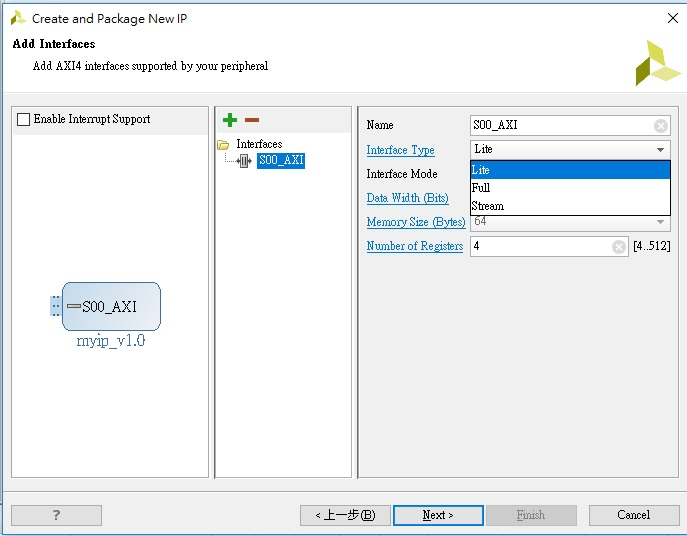
\includegraphics[scale=0.7]{images/register_type.jpg}
  \caption[Register types in Vivado]{Register types in Vivado}
  \label{fig:Register types in Vivado}
\end{figure}

These three types follow the protocol defined in AXI bus interface, and in our observation, UIO driver is working if we choose first two types, the thing goes wrong when we choose the third type ``Stream'' type. In \textbf{AXI reference guide} \cite{axiref}, we find that lite and full register follow the AXI4-Lite and AXI4 protocol, these protocols need to send the memory address when we transfer data. We can consider AXI4-Lite protocol is an easy-setting but function-restricted version of AXI4 protocol. While the stream register which follows the AXI4-Stream protocol is totally different, it does not need to specify the memory address and is a unidirectional channel. That is, in practical, if we want to read and write operation, we need at least two channels. This kind protocol is obvious that it can't be recognized in operation system as system memory.

Now we can finally conclude why UIO driver doesn't work on some IPs with DMA, because AXI4-Stream is a special bus protocol which is not compatible with the AXI4 bus protocol. Figure~\ref{fig:Custom IP with AXI4-Lite/Full Register.} and Figure~\ref{fig:Custom IP with DMA and AXI-Stream Register.} show the difference of two designs. So, if we want to use UIO driver to control our custom AXI4-Stream IP, we need to adapt UIO driver to control the DMA controller so that we can use it to submit DMA transaction to our IP.

We have modeled the high-level problem and proposed a possible solution, but there still has some concerns. How do we submit DMA transaction through UIO to DMA controller? Is there any problem when doing the DMA transaction? 


\newpage
\begin{figure}[!htb]
  \centering
  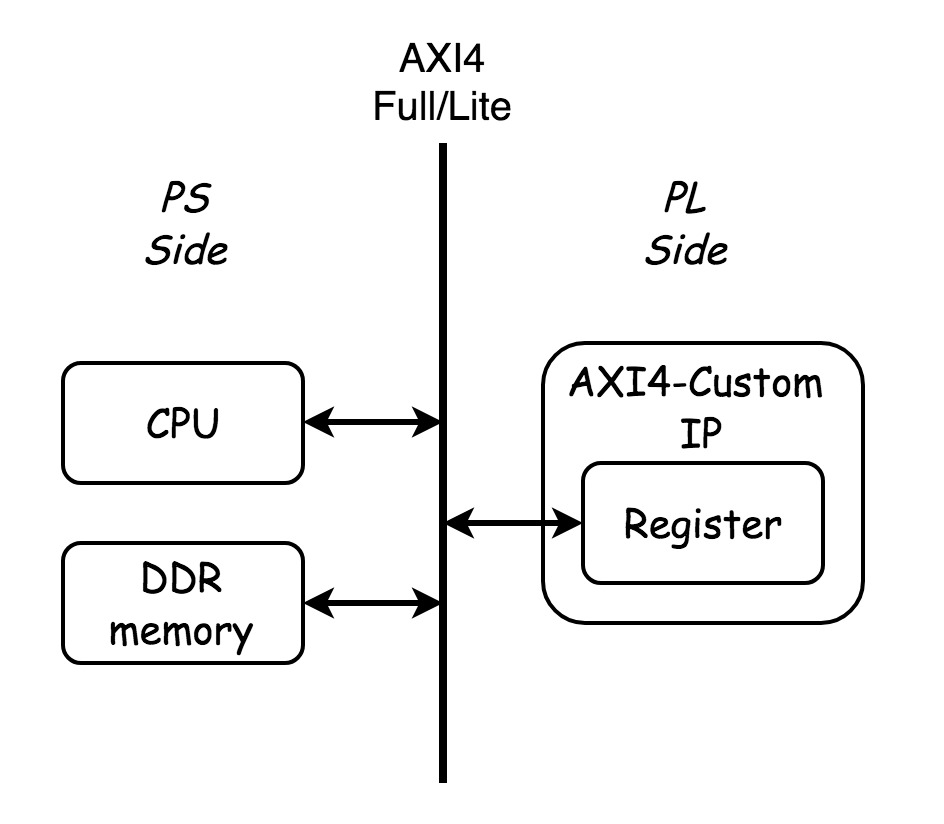
\includegraphics[scale=0.3]{images/customAXI4IP.jpg}
  \caption[Custom IP with AXI4-Lite/Full Register.]{Custom IP with AXI4-Lite/Full Register.}
  \label{fig:Custom IP with AXI4-Lite/Full Register.}
\end{figure}

\begin{figure}[!htb]
  \centering
  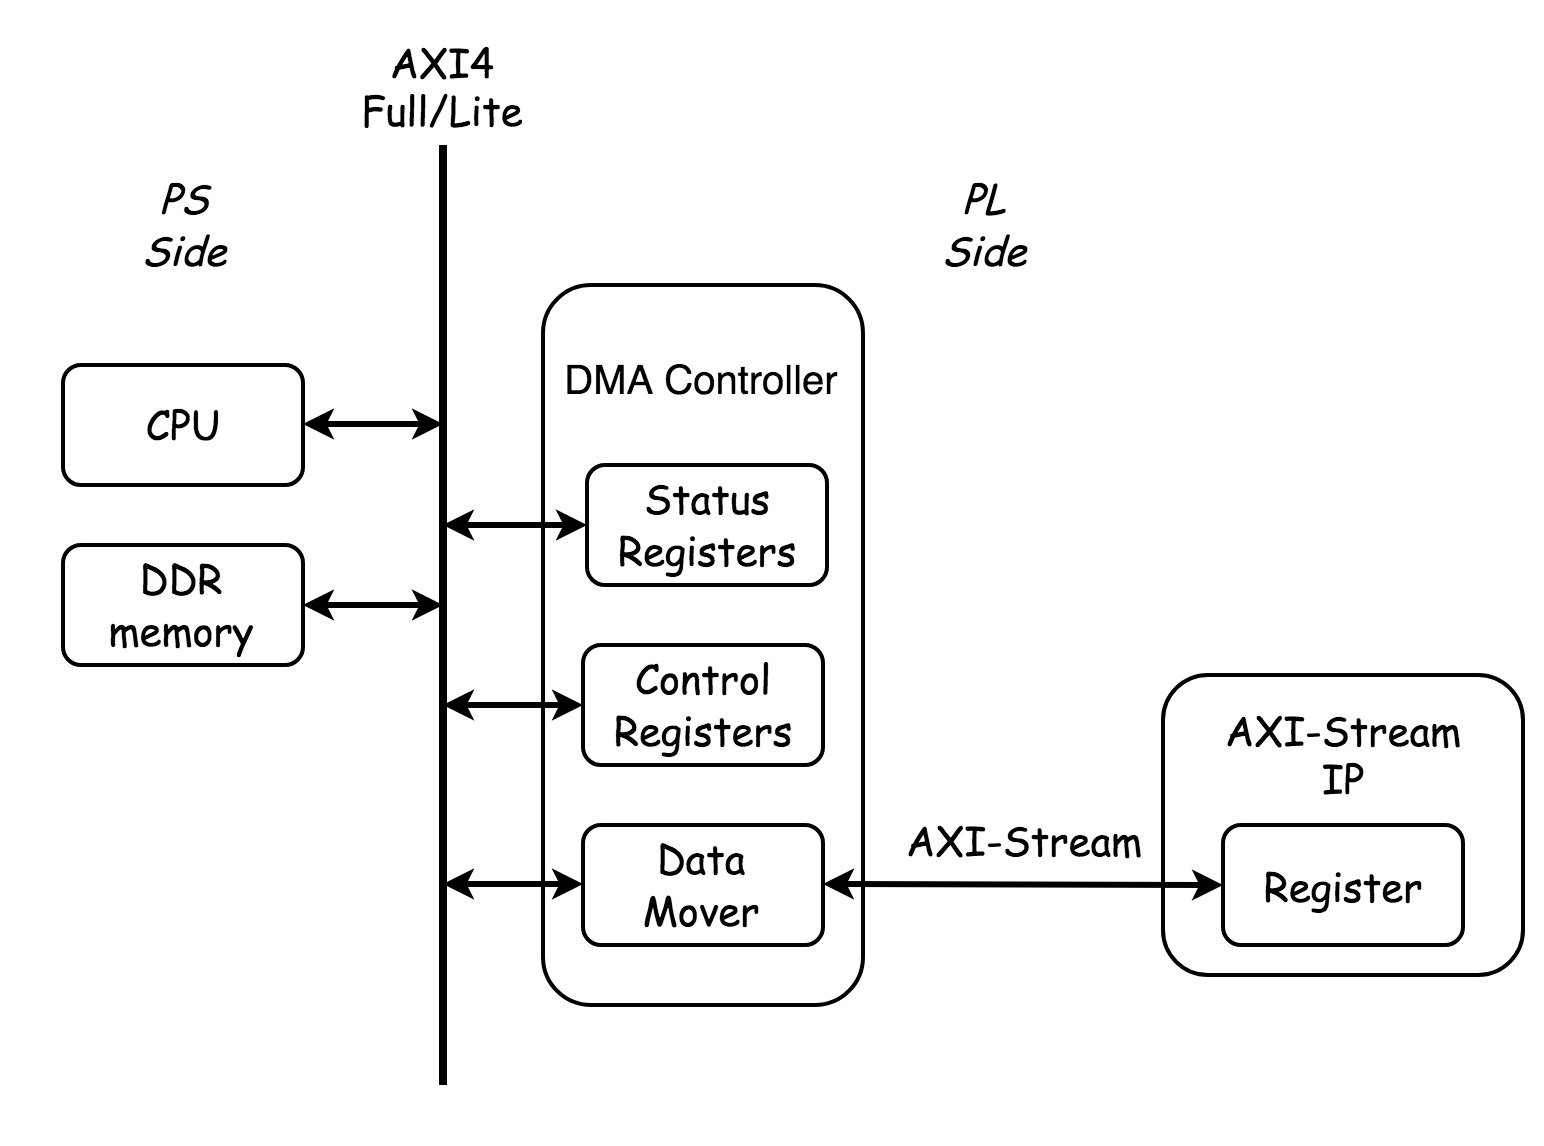
\includegraphics[scale=0.3]{images/customStreamIP.jpg}
  \caption[Custom IP with DMA and AXI-Stream Register.]{Custom IP with DMA and AXI-Stream Register.}
  \label{fig:Custom IP with DMA and AXI-Stream Register.}
\end{figure}
 

%-------------------------------------------------------------------------
% Section: 圖表
%-------------------------------------------------------------------------
\section{Problems}
\label{sec:Problems}

In this section, we will talk about File Operations, Continuous Memory For DMA, and Cache Coherency. We will explain these problems and show how we solve these problems in the following subsections.

\subsection{File Operations.}
\label{subsec:File Operations}
Let's see a simple example of controlling custom AXI4-Full/Lite IP with UIO,

{\renewcommand\baselinestretch{0.8}\selectfont
\begin{lstlisting}[frame=single,language=C]
int main(void)
{
  int fd = open("/dev/uio0", O_RDWR);
  void *ptr = mmap(0, 0x10000, PROT_READ|PROT_WRITE, MAP_SHARED, fd, 0);
  volatile uint32_t *ctrl = (uint32_t *)ptr;
  *ctrl = 0x00000000;
  ...
}
\end{lstlisting}
\par}
Typically, we open the device node to get device register pointer and memory-map to user memory, then we assign the value to those memory address to control the registers. Please note that, we need file operations to communicate with DMA in UIO driver, but in origianl scenario, we only use \textbf{mmap()} and the following value assignment has nothing to do with UIO driver. We need to find some file operations as a function entry. 


\subsection{Continuous Memory For DMA}
\label{subsec:Continuous Memory For DMA}
In traditional DMA transaction, it can only accept a contiguous (nonsegmented) block of
physical memory, so, if we want to use DMA in userspace, and we can not get a contiguous 
memory space(like CMA), 




\subsection{Cache Coherency}
\label{subsec:Cache Coherency}
While using DMA to do the data transfer, it may lead cache coherency problems. If we want to receive data to the buffer through the DMA, but the buffer is in cache now, to apply transaction, we give controller the buffer address and length. Once the transaction is done, we read the buffer and the value is the same as old value. CPU think the value in memory is not changed because whole data transfer is through DMA controller, so CPU keeps the old buffer data in the cache, that makes the difference between cache data and real data. Figure~\ref{fig:Cache Coherency Problems.} shows the cache coherency problem, both read and write may lead to this problem, so if we want to transfer the correct data, we must solve this problem.
\begin{figure}[!htb]
  \centering
  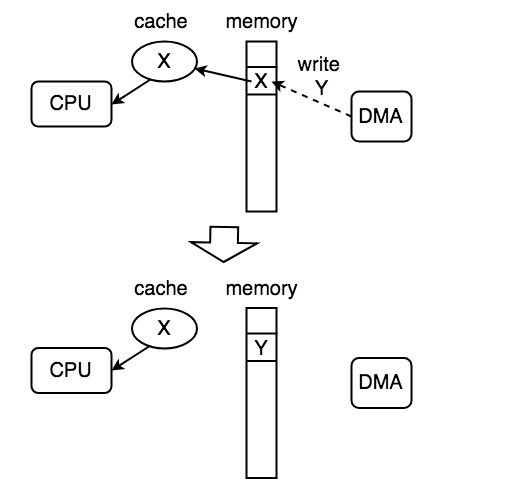
\includegraphics[scale=0.5]{images/cache_coherency.jpg}
  \caption[Cache Coherency Problems.]{Cache Coherency Problems.}
  \label{fig:Cache Coherency Problems.}
\end{figure}
\newpage
%-------------------------------------------------------------------------
% Section: 圖表
%-------------------------------------------------------------------------
\section{Linux UIO driver for AXI DMA}
\label{sec:Linux UIO driver for AXI DMA}
This sections will demonstrate our main work and explain how we solve the problems we have mentioned in previous section.

Let's take a look at two file operations \textbf{write(), read()} in UIO. Figure~\ref{fig:UIO write and read functions.} shows what these two functions doing, basically, these two functions in UIO driver is the handle about interrupt control. However, in our design, the UIO node is actually a virtual device node, so interrupt control and memory mapping are no more needed. That means we can use \textbf{write(), read()} to do the \emph{\textbf{real}} read/write, that is, Figure~\ref{fig:UIO write and read functions(modified)}. 

%\newpage
\begin{figure}[!htb]
  \centering
  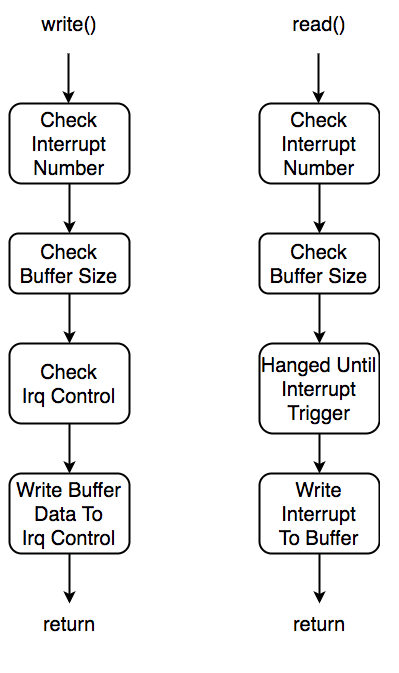
\includegraphics[scale=0.5]{images/uio_func_write.png}
  \caption[UIO write/read functions.]{UIO write/read functions}
  \label{fig:UIO write and read functions.}
\end{figure}

\begin{figure}[!htb]
  \centering
  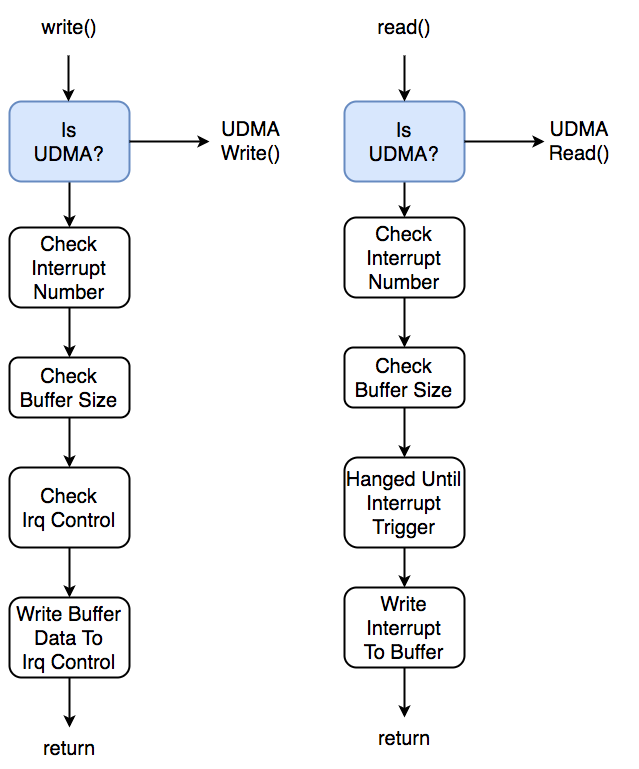
\includegraphics[scale=0.5]{images/udma_func_entry.png}
  \caption[UIO write/read functions(modified)]{UIO write/read functions(modified)}
  \label{fig:UIO write and read functions(modified)}
\end{figure}


\newpage
To solve the continuous memory issues, we apply DMA Scatter Gather mode. This mode allows non-contiguous (nonsegmented) block of physical memory and this mode need to turn on in Vivado 
design first. In this mode, DMA controller automatically gives the start address of the 
segmented of memory after the previous transaction of segmented memory is completed. To 
apply this mode, we need to construct a special data structure, Scatterlist, which collects 
start address and lengths of the segmented block of user buffer memory. DMA engine will do the
transaction according to this list. 

To avoid cache coherency problem, if transaction direction is memory-to-device, we need to flush 
cache to memory before submitting a transaction, if the direction is device-to-memory, we need to invalidate 
the cache after the transfer and before the CPU accesses memory. 
{}
%\newpage
These two problems will be considered in ``udma prepare dma'' shows in Figure~\ref{fig:UDMA write and read functions.}
In ``udma prepare dma'' function, we first \textbf{construct the scatterlist}, and call dma\_map\_sg() API provided by DMA engine to deal with the cache coherency problem in \textbf{Map the Scatterlist} stage. After all these settings, we can submit our DMA transaction to DMA controller, the following process is just like we have discussed in Section~\ref{sec:DMA}. Figure~\ref{fig:Udma Prepare for DMA} illustrates the stages in UDMA\_prepare\_DMA() function.

\begin{figure}[!htb]
  \centering
  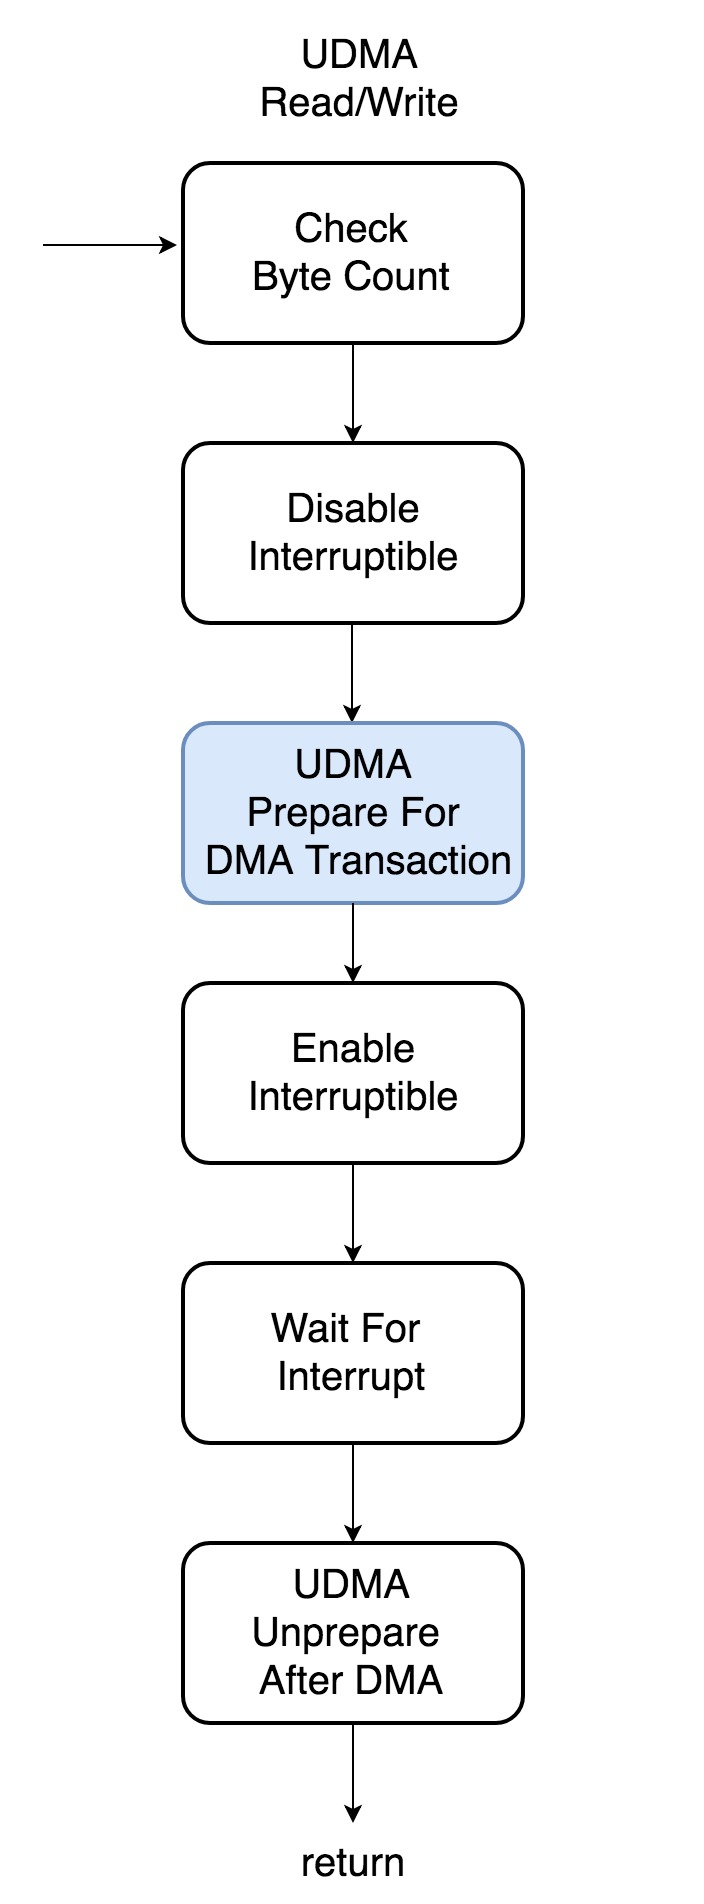
\includegraphics[scale=0.2]{images/udma_func.jpeg}
  \caption[UDMA write/read functions.]{UDMA write/read functions}
  \label{fig:UDMA write and read functions.}
\end{figure}

\begin{figure}[p]
  \centering
  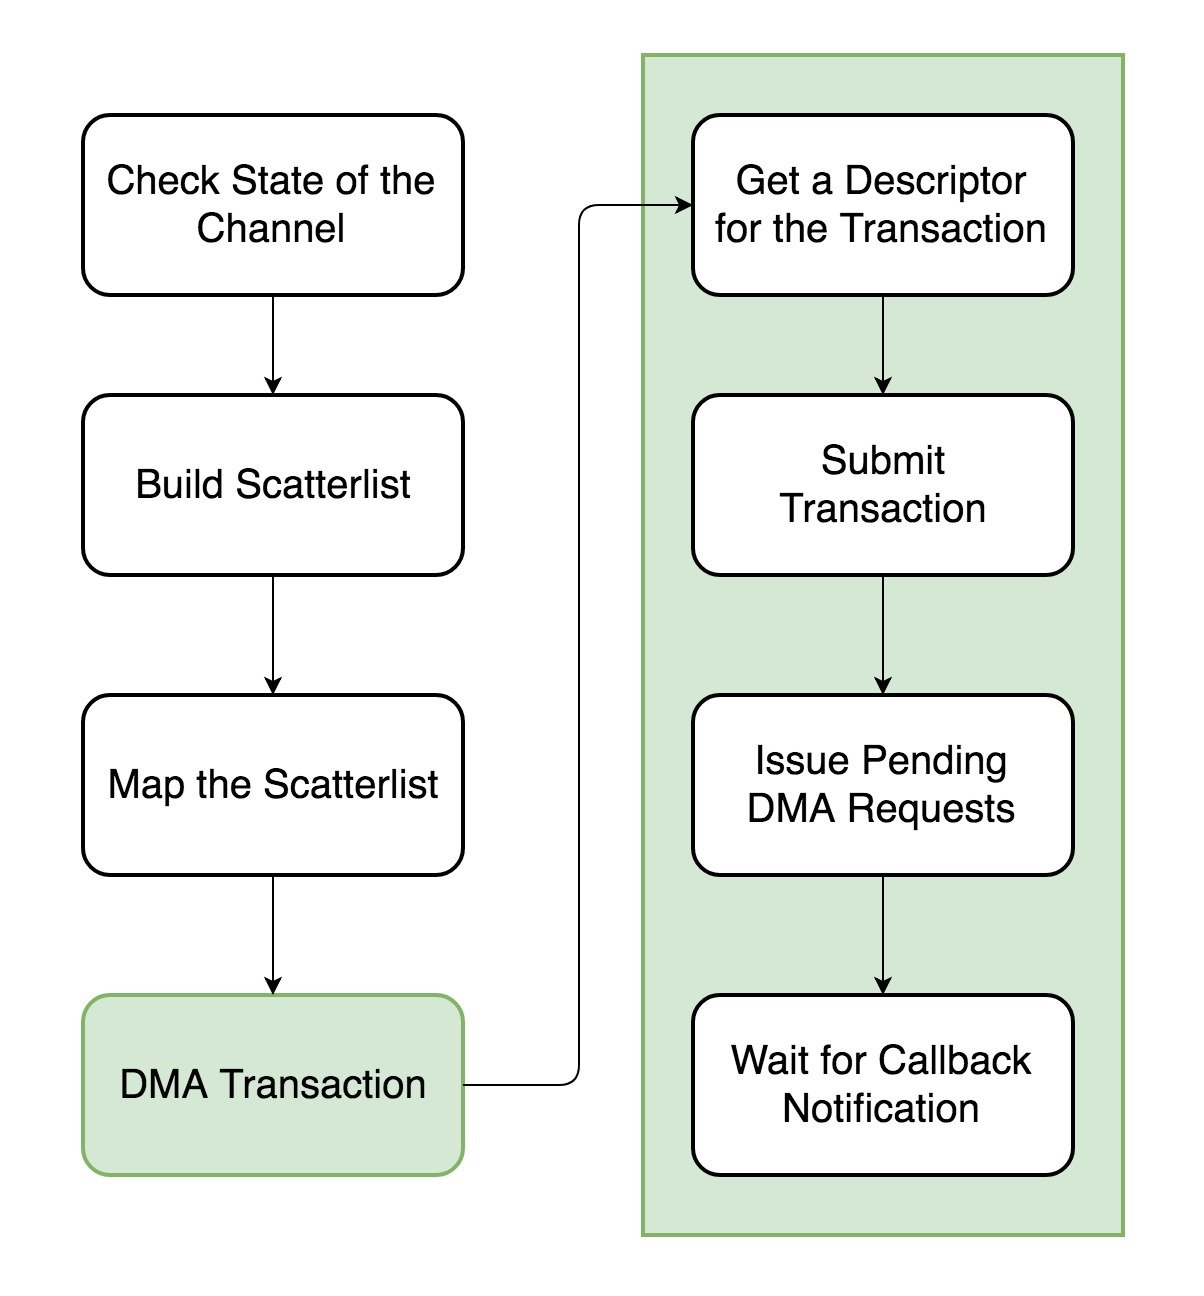
\includegraphics[scale=0.3]{images/udma_prepare_dma.jpg}
  \caption[Udma Prepare for DMA]{UDMA prepare for dma}
  \label{fig:Udma Prepare for DMA}
\end{figure}
\newpage

%-------------------------------------------------------------------------
% Section: Implementation
%-------------------------------------------------------------------------

\section{Implementation}
\label{sec:Implementation}
In this section, we will give a simple tutorial on how to use our new UIO driver and some settings. The entire design environment will be shown in Chapter 4. The full details of usage and code will be uploaded to GitHub repository\cite{mainwork}. 


\subsection{Device Tree File Format}
\label{subsec:Device Tree}
First, we need to set our virtual device in our device tree file, in AXI4 IP, we have device block looks like:

{\renewcommand\baselinestretch{0.8}\selectfont
\begin{lstlisting}[frame=single,language=C]
my_customIP@43c00000 {
	compatible = "generic-uio";
	reg = <0x43c00000 0x10000>;
	interrupts = <0 29 1>;
	interrupt-parent = <0x3>;
	xlnx,s00-axi-addr-width = <0x6>;
	xlnx,s00-axi-data-width = <0x20>;
}
\end{lstlisting}
\par}

It contains IP name, IP register address, register length, interrupt control...etc. These are essential properties if you want to apply a driver to control the device. But in our design, we have no real device, so the device node will look like:

{\renewcommand\baselinestretch{0.8}\selectfont
\begin{lstlisting}[frame=single,language=C]
udma0 {
    compatible = "generic-uio";
    dmas = <dma-channel1 dma-channel2>;
    dma-names = "loop_tx", "loop_rx";   
    ezdma,dirs = <2 1>;                 
};
\end{lstlisting}
\par}

Where dmas property refers to the DMA channel under ``axidma'' in device tree, for example, if ``axidma'' looks like:

{\renewcommand\baselinestretch{0.8}\selectfont
\begin{lstlisting}[frame=single,language=C]
loopback_dma: axidma@40410000 {
    #dma-cells = <1>;
    compatible = "xlnx,axi-dma";
    reg = < 0x40410000 0x10000 >;
    xlnx,include-sg;
    loopback_dma_mm2s_chan: dma-channel@40410000 {
        compatible = "xlnx,axi-dma-mm2s-channel";
        interrupt-parent = <&gic>;
        interrupts = <0 31 4>; 
        xlnx,datawidth = <0x20>;        
        xlnx,sg-length-width = <14>;    
        xlnx,device-id = <0x1>;     
    };
	loopback_dma_s2mm_chan: dma-channel@40410030 {
        compatible = "xlnx,axi-dma-s2mm-channel";
        interrupt-parent = <&gic>;
        interrupts = <0 32 4>;  
        xlnx,datawidth = <0x20>;       
        xlnx,sg-length-width = <14>;    
        xlnx,device-id = <0x1>;    
    };
};
\end{lstlisting}
\par}

Then ``dmas'' should be ``<\&loopback\_dma 0 \&loopback\_dma >'', dma-names is fixed in the driver, please make sure the names are the same as the setting. ``dirs'' tells the driver the direction of DMA channel. If the direction is not the same as the declaration in ``axidma'', it will fail when UIO is probing. ``mm2s'' means ``memory map to stream'', represents for the tx channel. ``s2mm'' means ``stream to memory map'' represents for the rx channel. After all these settings, our UIO driver should probe the device correctly and create a device node under /dev, like /dev/uio0.

\subsection{Compile New Kernel}
\label{subsec:Compile New Kernel}
Because we modified the UIO driver and add some new library in Linux kernel, we need to compile a new kernel. First, replace the old ``uio.c'' and ``uio\_pdrv\_genirq.c'' with new files. Then put ``udma.c'' under ``drivers/uio'' folder, and ``udma.h'' under ``include/linux'' folder. We need to add ``obj-y\  += udma.o'' in Makefile under ``drivers/uio'' . After, we can compile our new kernel with new UIO driver which can support DMA functions.

\subsection{Environment Variables Settings in U-boot}
\label{subsec:Linux On FPGA}
Same as the we mentioned in Chapter 2, we boot Linux on FPGA from SD card with two partitions. The boot files in first partition have much changed in our scenario, ``devicetree.dtb'' and ``uImage'' we have discussed in former subsection. The modification in ``uEnv.txt'' is quite easy, this file provides additional environment variables for the bootloader, u-boot. It will look like: 

{\renewcommand\baselinestretch{0.8}\selectfont
\begin{lstlisting}[frame=single,language=C]
bootargs=console=ttyPS0,115200 root=/dev/mmcblk0p2 rootwait rw earlyprintk uio_pdrv_genirq.of_id=genric-uio
...
\end{lstlisting}
\par}
To combine driver and device, please make sure that the string behind ``uio\_pdrv\_genirq.of\_id=''(in this case, is ``generic-uio'') is same as the property ``compatible'' of UIO node in device tree file.

\begin{figure}[!htb]
  \centering
  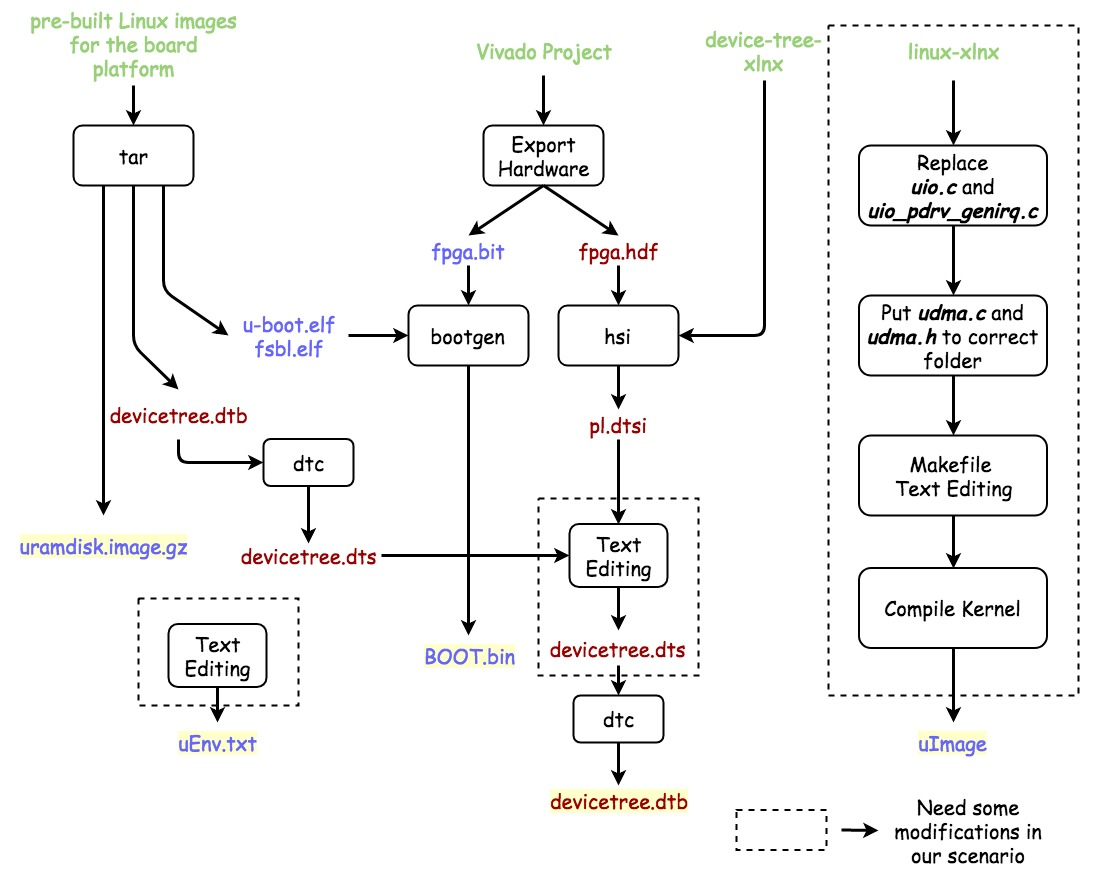
\includegraphics[scale=0.4]{images/new_embedded_linux.jpg}
  \caption[Embedded Linux on FPGA(UDMA ver.)]{Embedded Linux on FPGA(UDMA ver.)}
  \label{fig:Embedded Linux on FPGA(UDMA ver.)}
\end{figure}

Figure~\ref{fig:Embedded Linux on FPGA(UDMA ver.)} gives a simple illustration of our scenario. Unlike having lots of changes in 1st partition of SD card, we keep 2nd partition as usual, this partition provides the root file system when we boot up our Linux, just keeps it as the same.
\newpage

\subsection{Example}
\label{subsec:Example}
We will demonstrate how to use our driver in C.

{\renewcommand\baselinestretch{0.8}\selectfont
\begin{lstlisting}[frame=single,language=C]
Example1:

#define PACKET_SIZE (2048)

uint8_t tx_buf[PACKET_SIZE];
uint8_t rx_buf[PACKET_SIZE];

int main(void)
{
  int fd = open("/dev/uio0", O_RDWR);
  rv1 = write(fd, tx_buf, PACKET_SIZE);
  rv2 =  read(fd, rx_buf, PACKET_SIZE);

}
\end{lstlisting}
\par}

First, we open the device node to get the device pointer, and if we want to write the data in tx_buf to the device, we call write() function. If we want to read the data in the device to the rx_buf, we call read() function. All three parameters are easy to understand in the above example, the first parameter is the device pointer, the second one is the buffer pointer and the third one is the data size. Please note that the data size is the number of bytes, so if you declare buffer as type \textbf{uint32_t} which is a 32-bit array then your PACKET_SIZE in function need to be multiplied by 4. 

{\renewcommand\baselinestretch{0.8}\selectfont
\begin{lstlisting}[frame=single,language=C]
Example2:

#define PACKET_SIZE (2048)

uint32_t tx_buf[PACKET_SIZE];
uint32_t rx_buf[PACKET_SIZE];

int main(void)
{
  int fd = open("/dev/uio0", O_RDWR);
  rv1 = write(fd, tx_buf, PACKET_SIZE *4);
  rv2 =  read(fd, rx_buf, PACKET_SIZE *4);

}
\end{lstlisting}
\par}

The return value is the number of bytes, basically, it is equal to the value of the third argument you put in the function.
In example1, rv1 and rv2 are 2048, in example2, rv1 and rv2 are 8192.